\documentclass[a4paper,twoside]{article}

\usepackage{epsfig}
\usepackage{subfigure}
\usepackage{calc}
\usepackage{amssymb}
\usepackage{amstext}
\usepackage{amsmath}
\usepackage{amsthm}
\usepackage{multicol}
\usepackage{pslatex}
\usepackage{apalike}
\usepackage{tabularx}
\usepackage{SCITEPRESS}
\usepackage[small]{caption}
\usepackage{url}

\subfigtopskip=0pt
\subfigcapskip=0pt
\subfigbottomskip=0pt

\begin{document}

\title{Testing the Differences of Using RGB and HSV Histograms During Evolution in Evolutionary Art}

\author{\authorname{P. Garc{\'i}a-S{\'a}nchez\sup{1}, J.J. Merelo\sup{1}, D. Calandria\sup{2}, A. B. Pelegrina \sup{3}, R. Morcillo, F. Palacio \sup{4}, R. H. Garc{\'i}a-Ortega \sup{4}}
%\affiliation{Secret Affiliation}
\affiliation{\sup{1}Dept. of Computer Architecture and Computer Technology and CITIC-UGR, ETS. Inform{\'a}tica y Telecomunicaci{\'o}n, University of Granada, Granada, Spain}
\affiliation{\sup{2}Proemium, Granada, Spain}
\affiliation{\sup{3}Department of Translation and Interpreting, University of Granada, Granada, Spain}
\affiliation{\sup{4}ETS. Inform{\'a}tica y Telecomunicaci{\'o}n, University of Granada, Granada, Spain}
\affiliation{\sup{4}Fundaci{\'o}n I+D del Software Libre, Granada, Spain}
\email{pgarcia@atc.ugr.es, jmerelo@geneura.ugr.es, dcalandria@proenium.com, abpelegrina@ugr.es, robermorji@gmail.com, fruela@correo.ugr.es, rhgarcia@ugr.es}
%\email{secret@anonymous.com}
}

\keywords{Evolutionary Art, HSV, RGB, Processing}

\abstract{%This paper shows how the Processing framework can be used to generate
%Evolutionary Art comparing HSV and RGB histograms of a test image. Processing is a framework created for visual
%insisto, ese no debería ser el objetivo del artículo. Seguro que hay
%cientos de papers que hacen ya eso. Hay que insistir en lo nuevo del
%artículo - JJ - FERGU: Le meto lo de los histogramas para que sean 2 cosas lo que vendemos
%designers and artists that is starting to have great presence in the
%interactive and visual art field. It includes several modules for
%image creation, manipulation and analysis. 
This paper compares the use of RGB and HSV histograms during the execution of an Evolutionary Algorithm. This algorithm generates abstract
images that try to match the histograms of a target image. Three different
fitness functions have been used to compare: the differences
between the individual with the RGB histogram of the test image, the
HSV histogram, and an average of the two histograms at the same
time. Results show that the HSV fitness also increases the similarities of the
RGB (and therefore, the average) more than the other two measures.  
}
% Mejora las similaridades del RGB? Será que es más similar que el RGB
% - JJ FERGU: El RGB y HSV representan lo mismo, pero no están relacionados linealmente (lo explico en el paper), pero usar HSV también hace que se parezca más el RGB}

\onecolumn \maketitle \normalsize \vfill

\section{\uppercase{Introduction}}
\noindent Evolutionary Art \cite{EART} is a branch of generative art \cite{PHEROGRAPHY} created using a
computer, following the principle of the survival of the fittest, % pero qué es "fittest" en este contexto? - JJ FERGU: Explicado a continuación
using Evolutionary Computation methods \cite{INTROEIBEN}. A population
of artistic works (individuals) are evaluated with an aesthetic
measure to yield a score (fitness). These individuals are combined and
mutated to generate an offspring with inherited properties of the
parents, during a certain number of times. 

There exist several metrics to score the generated images, such as opinion from humans, or image characteristics (for example, specific combination of colours). The main goal of this paper is to study the differences of using
the information of the HSV (Hue, Saturation, Value) and RGB (Red,
Green, Blue) histograms during the evolution. Although the two histograms represent the same information, using HSV (instead as RGB) as a color model increases the accuracy in image retrieval and indexing, as explained in \cite{COLORDIFFERENCES}. The results of this investigation can help in future evolutionary art algorithms, adding the most appropiate color model feature with other features available in the literature. For example, to be used as one of the features of any kind of classifier.
%The secondary goals is to test the advantages of using
% Ese no es el objetivo del trabajo, a menos que realmente pruebes que
% Processing es mejor que alguna otra alternativa - JJ - Fergu: por eso es uno de los goals, pero he cambiado el orden, ahora esto es lo importante
%Processing \cite{PROCESSING}, a programming framework designed for visual artists, in
%Evolutionary Art. 
In this work the Processing \cite{PROCESSING} framework is used inside an Evolutionary Algorithm (EA) to model the
individuals, generate their associate images and extract information
of them (HSV, RGB and Average histograms) to fit with the histograms
of a test image. Processing has been integrated in the OSGiLiath \cite{OSGILIATH} 
evolutionary framework to take advantage of the capabilities offered in image manipulation and analysis.
% Este sí podría ser el objetivo del trabajo - JJ FERGU: Cambiado arriba el orden


% Deberíais incluir un apartado un poco más extenso de
% motivación. ¿Qué interés tiene hacer esto? ¿Qué contexto? ¿Es para
% probar que es muy fácil añadir cosas a Osgiliath? Habla de Osgiliath
% también y lo que significa - JJ FERGU: Añadido. Eso lo explico también en la sección Setup

The rest of the work is organized as follows: in Section \ref{sec:soa}, a brief review on Evolutionary Art is presented. Processing framework and image information are described next (Section \ref{sec:processing}). The experimental setup and results are presented in Sections \ref{sec:setup} and \ref{sec:results}, respectively. Finally, the conclusions and future work can be found in Section \ref{sec:conclusions}.

\section{\uppercase{STATE OF THE ART}}
\label{sec:soa}
\noindent Computational Aesthetics ``is the research of computational methods that can make applicable aesthetics decisions in a similar fashion as humans can'' \cite{COMPAESTH}. In the field of computational aesthetics, evolutionary systems can play an important role, by enabling the evolution of aesthetically pleasing or innovative structures \cite{dipaola2009incorporating}. Evolutionary art is characterized by the use of evolutionary principles and natural selection as a generative process. One of the earliest applications of evolutionary systems to generate art is the proposal of Sims to use an EA to create complex images \cite{sims1991artificial} or virtual creatures  \cite{sims1994evolving}. In evolutionary art systems, the evaluation of the aesthetics can be done using human feedback, with some interactive evaluation of the population, such as \cite{ashlock2006evolutionary,draves2006electric,moroni2000vox} and \cite{sims1991artificial}. It also can be achieved by using an automatic evaluation of fitness, as presented in \cite{aguilar2008robotic,den2010comparing,dipaola2009incorporating,li2012investigating}, and \cite{sims1994evolving}.

One of the main challenges in Evolutionary Art is how to measure aesthetic value of a piece of evolutive art. The source of this difficulty lies in the inherent complexity, subjectivity and dynamism of aesthetics. Nevertheless, a wide number of metrics has been presented. According to \cite{galanter2012computational}, these measures can be classified into several categories in several pieces of research. The first category involves the evaluation of the aesthetics of a piece of art by a formula or principle (e.g., pythagorean proportions). Other measures apply certain principles of design, such as the rule of thirds or color theory (e.g., using complimentary colors in Pop Art \cite{den2012evolving}), neural networks or complexity measures. 

This classification also provides a sub-classification for evolutionary systems. First, it identifies interactive evolutionary systems, where the fitness of the individuals is determined by human agents. Another category is performance based goals: certain properties of the art piece are evaluated and optimized based on performance measures (e.g., usable surface in a furniture design generator). Other systems use an exemplar (i.e., real world example) as a way to measure the fitness of the individuals. Finally, some models use the idea that the complexity is directly related to aesthetics and follow the path firstly stablished in \cite{birkhoff2003aesthetic}.  Given the multidimensional nature of aesthetics judgement, multi-objective EAs are a straightforward option to deal with this multidimensionality. Other extensions to EA, like coevolution or agent swarm behavior, can be used in evolutionary art systems.

A brief classification of the aesthetic measures found in the evolutionary art systems mentioned in the previous paragraph is shown in Table~\ref{table_class}.

\begin{table*}[!t] 
\renewcommand{\arraystretch}{1.3} 
\caption{Classification of the aesthetic measures used in a brief review of the literature on evolutive art.} 
\label{table_class} 
\centering
\begin{tabularx}{\textwidth}{|l|X|}
\hline
Type & Aesthetic Measure \\ \hline
Formulaic and Geometric Theories & Fractal dimension \cite{den2010comparing}, Image order \cite{li2012investigating}, Benford Law \cite{del2005benford}\\ \hline
Based on Design Principles &  Color contrast (hue) \cite{den2012evolving},  Color ingredient \cite{li2012investigating}, Composition, tonality and color \cite{dipaola2009incorporating}.\\ \hline
Interactive Evolutionary Computation & The electric sheep project \cite{draves2006electric} \cite{ashlock2006evolutionary,moroni2000vox}\\ \hline
Error relative to Exemplars &  Resemblance score \cite{dipaola2009incorporating}, pixel comparation \cite{aguilar2008robotic}\\ \hline
Performance based goals & Evolving virtual creatures \cite{sims1994evolving} \\\hline
Complexity measures & Image complexity \cite{li2012investigating}, Machado and Cardoso aesthetic measure \cite{machado1998computing}\\ \hline
\end{tabularx}
\end{table*}

Several methods for the representation of the art in evolutionary art have been proposed. In symbolic expression, the genotype is a tree of expressions and the phenotype consists in the image produced  by the evaluation of the tree. Shape grammars can also be used as a formal description of the image. Previously existing images can be used as a basis for the evolution process. Finally, other representations can be based on mathematical models, like fractals or cellular automata.


%\rowcolors{2}{gray!25}{white}


\section{PROCESSING AND HISTOGRAMS}
\label{sec:processing}
\noindent In this section we describe Processing \footnote{\url{http://www.processing.org/}} and the histograms used. Processing \cite{PROCESSING} is a framework formed by a simple programming language and an integrated development environment (IDE) primarily created for electronic and visual artists, designers, musicians, etc. Processing offers the following advantages:

\begin{itemize}
\item Processing was created for artists, rather than programmers. So, it allows very complex drawings and interactive applications with few lines of code.
\item It is an Open Source software (licensed under the GNU Lesser General Public License), and counts with a large development community.
\item It is based on OpenGL, thus providing 3D acceleration.
\item It also includes more than 100 libraries for video, sound, physics, computer vision, networking, etc.
\item Easy integration with Java, HTML5 and Android.
\end{itemize}

%\begin{figure*}[ht]
%\centering

%\subfigure[Processing IDE]{
%   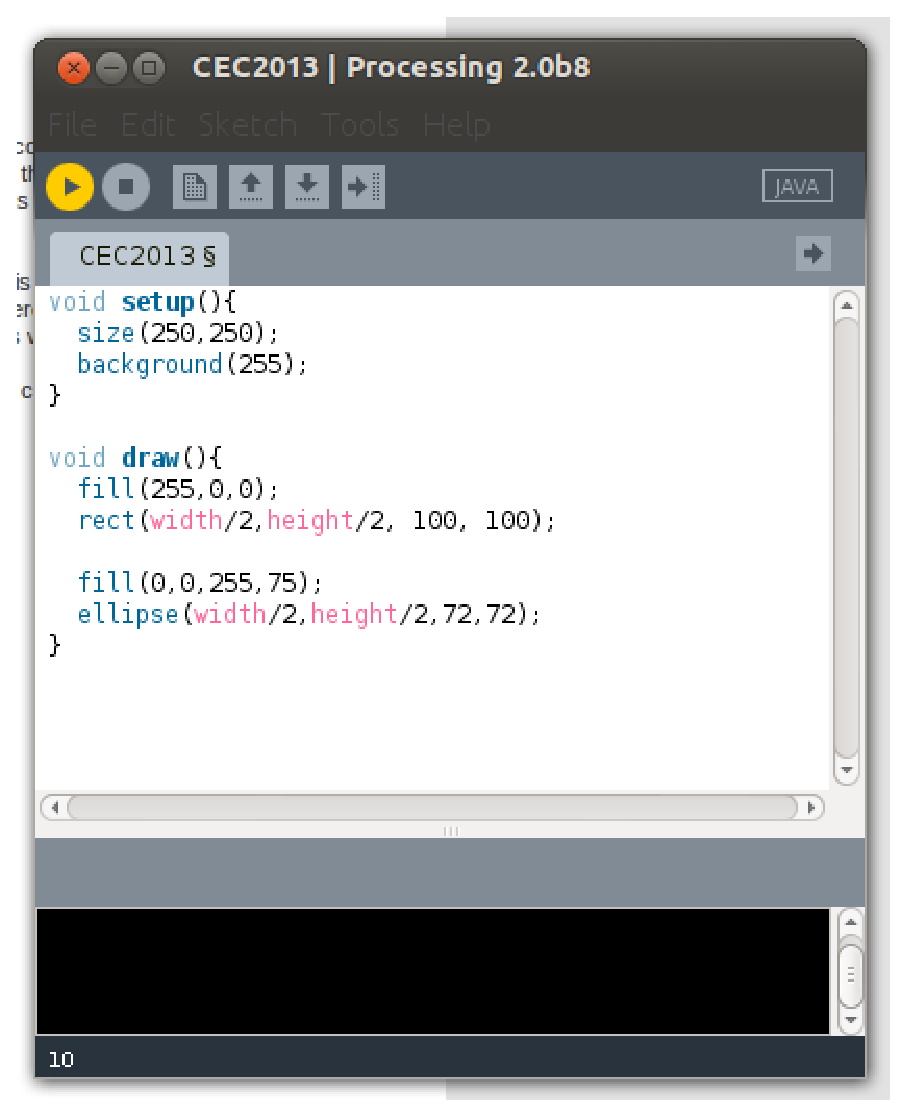
\includegraphics[scale =0.55] {images/Processing.eps}
%   \label{fig:subide}
% }
%\subfigure[Runtime of the code.]{
%   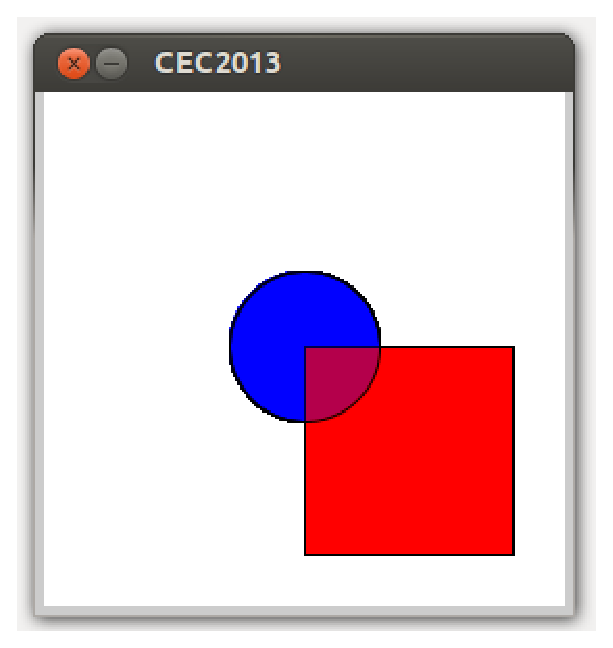
\includegraphics[scale =0.45] {images/run.eps}
%   \label{fig:subsketch}
% }

%\label{fig:ide}
%\caption{Processing IDE and sketch execution. }
%\end{figure*}

However, being a light framework, there exist some disadvantages:
\begin{itemize}
\item More complex applications require more programming skills.
\item The calculations of large computer images are a bit inefficient (although expert programmers can manage OpenGL at low level to fix this).
\end{itemize}

There exist a lot of interactive artistic projects made with Processing; examples include art generation, artificial life, interactive music and other. A good selection can be seen in \url{http://processing.org/exhibition/}.

%Processing is composed by several modules:

%\begin{itemize}
%\item Structure: Includes typical programming functions as is the case of return, draw, void, and everything related to the structure of the program.
%\item Environment: Formed by the functions that handle the modeling of the window: cursor, width, height, background, for example.
%\item Data: formed by the data types that make up the different program variables (int, char, float).
%\item Control: Consisting in relations operators.
%\item Shape: it is formed by all functions of the treatment of figures 3D and 2D.
%\item Input: input interactivity features such as functions for the mouse, keyboard or files.
%\item Output: output interactivity features such as write on the screen, save the image or serial control.
%\item Transform: transformations such as rotations or translations.
%\item Lights and Cameras: Functions for the treatment of the lights and cameras.
%\item Color: Functions to handle color of the figures.
%\item Image: Functions for loading images or textures.
%\item Rendering: Functions for rendering images.
%\item Typography: Functions for dealing with text.
%\item Math: Functions for dealing with all mathematical functionality.
%\end{itemize}

The Color module can be used to analyze images taking into account their histogram. The color histogram represents the frequency of occurrence of each color intensities present in the image, by accounting for such sharing pixels color intensity values.

The histogram is composed of different ranges or bins that represent a value or set of values of color intensity. The color space is defined as a model representation with respect to color intensity values. Two color models are used in this paper: RGB (Red, Green, Blue) and HSV (Hue, Saturation and Value). The RGB model is an additive color model in which red, green and blue are added together in different proportions to reproduce a wide range of colors, while the HSV is based on hue or tone, saturation and brightness. While the RGB model is the closest to the way color is processed in some machines, the HSV representation provides a more accurate way to model how humans perceive colors, and also provides more information in image retrieval \cite{COLORDIFFERENCES}.
Figure \ref{fig:histogram} shows the RGB histogram of the image in Figure \ref{fig:flevopark} (photo taken by the first author).

\begin{figure}
\centering
   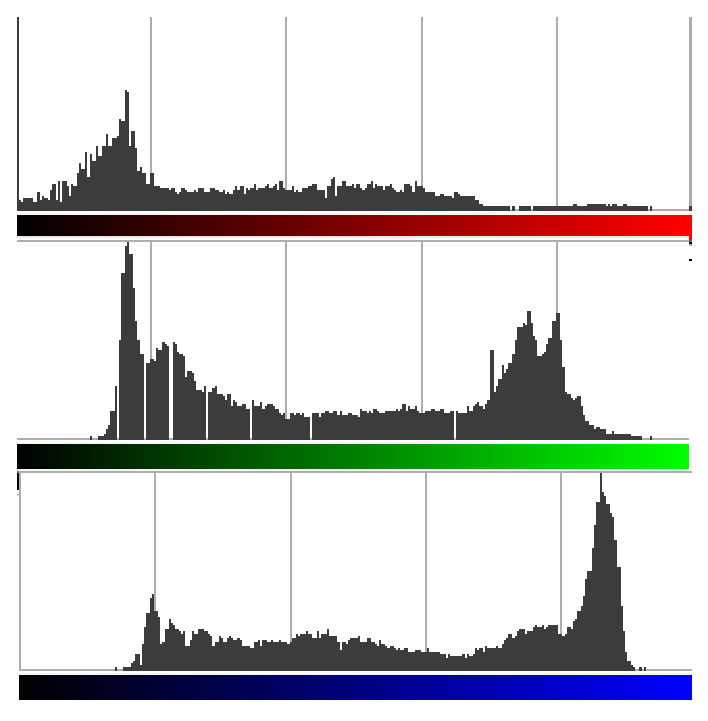
\includegraphics[scale =0.6] {images/histogram.eps}
\caption{RGB histogram of Figure \ref{fig:flevopark}. }
\label{fig:histogram}
\end{figure}

\begin{figure}
\centering
   
\includegraphics[scale =3] {images/flevopark.eps}
\caption{Test image to compare with the Fitness functions of our algorithm.}
\label{fig:flevopark}
\end{figure}

\section{EXPERIMENTAL SETUP}
\label{sec:setup}

\noindent This section shows how Processing has been used in the EA, the individual representation, the fitness functions, and the parameters of the experiments.

\subsection{Integrating Processing in Java}
Processing can be integrated with Java just by adding a {\em jar} (a Java library) to existing software. In this work, Processing has been integrated to an existent EA framework, OSGiLiath \cite{OSGILIATH}, a service-oriented framework based on Java that includes a lot of primitives and services for Evolutionary Computation. A new module called OSGiLiART has been added to the publicly-available source code of OSGiLiath (available in \url{http://www.osgiliath.org}) under a LGPL License. Then, using the packages available in the Processing library the EA can generate individuals, manipulate images or extract information.

\subsection{Individual Representation}

To perform the experiments, the genome of the individual is a list of circles. Each circle has a position, radium and color. This list can be recombined or mutated (changing the color, position or radium of a circle of the list).

\subsection{Fitness Used}
For this piece of research, we focused on the aesthetics measure of histogram comparison. The fitness functions are included in the ``Error relative to Exemplars'' category, using Galanter \cite{galanter2012computational} classification. The idea is to obtain an image with the same proportion of tones and colors of a aesthetical existent image.

Three different fitness functions have been tested:
\begin{itemize}
\item {\em RGB difference}: The difference of the RGB histogram of the individual with the RGB histogram of the test image.
\item {\em HSV difference}: The difference of the HSV histogram of the individual with the HSV histogram of the test image.
\item {\em Average difference}: An average of the two previous differences.
\end{itemize}

The range of the these fitness function has been normalized to vary from 0 (totally different histograms) to 1 (the same histogram).

%\subsubsection{Histogram comparision}\label{go:fitness:hist}
For every color property (i.e., RED, GREEN, BLUE, HUE, SATURATION and VALUE), the histogram is computed using the expression (\ref{eq:histogram}) for each possible value (0-255). Then, again for every property, the difference between the target image and the individual histograms is obtained using (\ref{eq:diff}). Finally, the three fitness are calculated: RGB fitness (\ref{eq:RGB}), HSV fitness (\ref{eq:HSV}) and AVERAGE fitness (\ref{eq:AVERAGE}).

\begin{eqnarray}
	\label{eq:histogram}
	H(c, prop) = \frac{1}{N}\sum_{j=0}^N \left\{\begin{matrix}
1 & prop(j) = c\\ 
0 & otherwise
\end{matrix}\right. \\
\label{eq:diff}
diff(h_1, h_2) = \sum_{j=0}^{255} |h_1(j) - h_2(j)|
\end{eqnarray}
\begin{eqnarray}
	d_R(i) = diff(H(i, RED), H(target, RED))\\
	d_G(i) = diff(H(i, GREEN), H(target, GREEN))\\
	d_B(i) =  diff(H(i, BLUE), H(target, BLUE))\\
	\label{eq:RGB}
	fitness_{RGB}(i) = 1 - 128\frac{d_R(i) + d_G(i) + d_B(i)}{3}
\end{eqnarray}
\begin{eqnarray}
	d_H(i) = diff(H(i, HUE), H(target, HUE))\\
	d_S(i) = diff(H(i, SAT), H(target, SAT))\\
	d_V(i) =  diff(H(i, VAL), H(target, VAL))\\
	\label{eq:HSV}
	fitness_{HSV}(i) = 1 - 128\frac{d_H(i) + d_S(i) + d_V(i)}{3}
\end{eqnarray}
\begin{eqnarray}
	\label{eq:AVERAGE}
	fitness_{AVERAGE}(i) = \frac{fitness_{RGB}+fitness_{HSV}}{2}
\end{eqnarray}


\subsection{Parameters Used}

A steady-state evolutionary algorithm has been used. Each individual is randomly generated at the initialization of the EA. The genome size is 50 elements (circles of maximum radium of 128 pixels). Population size has been set to 32 individuals. Uniform crossover rate is 0.5, and a binary tournament has been chosen for selection (that is, a pool of 16 parents is selected and crossed). Mutation probability is 0.04 (the usual value of {\em 1/genomesize}). Finally, the image size for each individual is 256x256 pixels. The individuals have been compared with the histograms obtained from the image of Figure \ref{fig:flevopark} to guide the evolution. 

\section{\uppercase{RESULTS}}
\label{sec:results}

\noindent Because of the stochastic nature of the EAs, each algorithm has been executed 30 times for each different fitness. Table \ref{tab:results} shows the average differences (and standard deviation) attained with each fitness used. As can be seen, using the HSV histogram differences as fitness produces a higher RGB similarity (and therefore, average) than using the RGB or Average fitness. However, using the average between the two histogram differences produces higher similarity in HSV (0.294) than only taking into account the HSV. The maximum fitness is around 25\% of similarity with the original image since the individual is a list of 50 circles, and therefore, only a maximum of 50 different colors are used (while in the original jpg image can be more than millions). See the histogram of a generated best individual by the algorithm in Figure \ref{fig:histoind}. An example of evolution for each fitness can be seen in Figure \ref{fig:rgbgens}, \ref{fig:hsvgens} and \ref{fig:averagegens}. Comparing with the RGB histogram as fitness, a bigger fluctuation in the HSV is produced (Figure \ref{fig:rgbgens}). This can be explained because the RGB information tends to be more noisy than HSV information: in fact, in \cite{COLORDIFFERENCES} authors explain the problems this histogram offers with respect to HSV in image retrieval. Although there is the same information modeled in both histograms, the transformation from one to another is not linear, so there is no relation with the histograms of individuals generated during the evolution.

\begin{table*}
\centering
\caption{Results for the different fitness (average of the 30 executions and standard deviation). Only one histogram type is used for fitness calculation, but the other values obtained are also added.}
\begin{tabular}{|c|c|c|c|} \hline
Differences used  in Fitness & Obtained RGB      & Obtained HSV  & Obtained Average \\ \hline
RGB Histogram    & 0.267 $\pm$ 0.012	& 0.170 $\pm$ 0.010 	& 0.218 $\pm$ 0.009	\\ \hline
HSV Histogram    & 0.227 $\pm$ 0.017	& 0.265 $\pm$ 0.021	& 0.246 $\pm$ 0.010 \\ \hline
Average Histogram& 0.173 $\pm$ 0.012	& 0.294 $\pm$ 0.013	& 0.234 $\pm$ 0.010 \\ \hline
\end{tabular}
\label{tab:results}
\end{table*}

\begin{figure}
\centering
   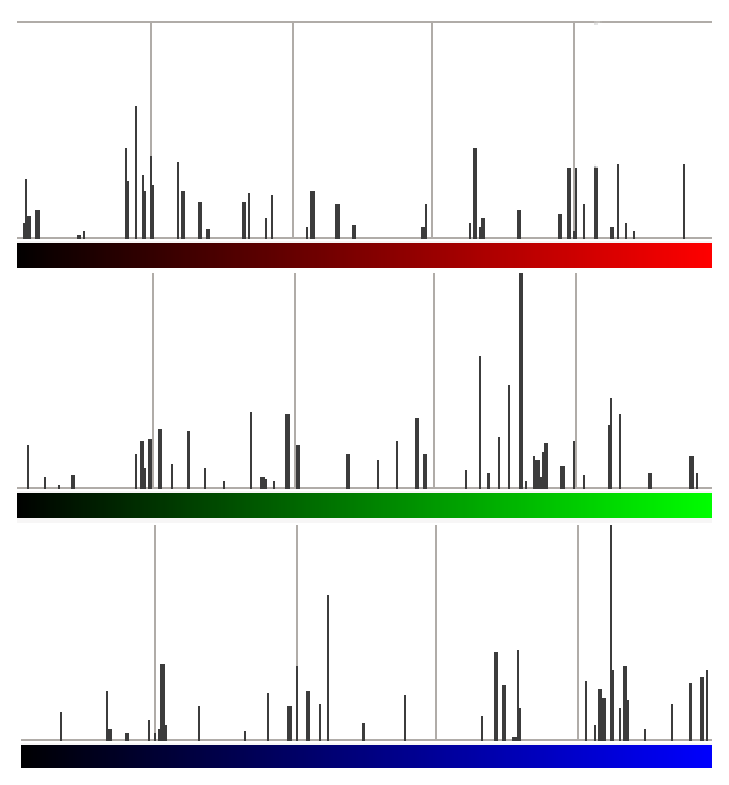
\includegraphics[scale =0.6] {images/individuohist.eps}
\caption{RGB histogram of a solution generated by the algorithm.}
\label{fig:histoind}
\end{figure}

\begin{figure}
   \includegraphics[angle=-90,scale =0.30] {images/rgbgens.eps}
\caption{Evolution of the difference in RGB histogram of the best individual compared with the test image. }
\label{fig:rgbgens}
\end{figure}

\begin{figure}
   \includegraphics[angle=-90,scale =0.30] {images/hsvgens.eps}
\caption{Evolution of the difference in HSV histogram of the best individual compared with the test image. }
\label{fig:hsvgens}
\end{figure}

\begin{figure}
   \includegraphics[angle=-90,scale =0.30] {images/averagegens.eps}
\caption{Evolution of the difference of average of RGB and HSV histogram of the best individual compared with the test image. }
\label{fig:averagegens}
\end{figure}

The best individuals attained are shown in Figure \ref{fig:bestinds}. Note that, although the numeric fitness is similar, they produce different color tones. This can be explained for the limitation of colors used in the individual representation, as previously said, or the noisy characteristic of the RGB histogram. Figure \ref{fig:collage} shows one evolution of the best individual using the HSV fitness in the first 64 generations.

\begin{figure*}[ht]
\centering
\subfigure[Best individual using RGB]{
   
\includegraphics[scale =0.5] {images/RGB.eps}
 }
\subfigure[Best individual using HSV]{
   
\includegraphics[scale =0.5] {images/HSV.eps}
 }
\subfigure[Best individual using AVERAGE]{
   
\includegraphics[scale =0.5] {images/AVERAGE.eps}
 }
\caption{Best individuals obtained with the three fitness used (HSV, RGB and AVERAGE).}
\label{fig:bestinds}
\end{figure*}

\begin{figure}
   \includegraphics[scale =0.10] {images/collage.eps}
\caption{Evolution of the best individual using the HSV histogram difference. }
\label{fig:collage}
\end{figure}

\section{\uppercase{Conclusions and Future Work}}
\label{sec:conclusions}
\noindent This paper introduces an Evolutionary Algorithm that uses the Processing framework to generate images and to extract image information using HSV and RGB histograms. %The advantages of this framework have been presented and we think that Evolutionary Art area can take advantage of them. 
In this work individuals are represented as a list of Processing primitives (circles) and the fitness functions used are based on the similarity with an existent aesthetic image. Three different fitness functions using color histogram have been tested: difference between the HSV and RGB histograms, and an average difference of the two histograms at the same time. Experiments show that better results in terms of similarity are obtained using the HSV comparison (due to the noisy information provided by the RGB). 

The future work for this research also includes more experiment with other kind of individuals, apart from circles: using other primitives, such as rectangles or triangles, for example. The use of textures and gradients will generate images with higher number of colors, obtaining more fidelity (more than 25\%) with the test image. Other metrics explained in previous sections will be also implemented. Finally, our intention is not only to create only static images, but use the Processing libraries to create evolutionary interactive art combining sounds and motion. A human guidance tool is also being developed to obtain human feedback to create a knowledge base for future experimentation (available in \url{http://evorq.ugr.es:8080/HumanGuidance}). The results will be gathered to create a database of different features to guide the evolution. More complex measurements will be studied in next works, taking into account that the HSV is the color mode that provides more information during the evolution, having less noisy behaviour.

The used software and algorithms presented are Open Source under a GPL license, and can be obtained from \url{http://www.osgiliath.org}.

\section*{\uppercase{acknowledgements}}
\noindent This work has been supported in part by FPU research grant AP2009-2942 and projects EvOrq (TIC-3903), SINECA (0100DGT21285, Spanish Direccion General de Trafico), TIN2011-28627-C04-02 and FFI2011-22397 (funded by Spanish Ministry for Economy and Productivity). This work was developed during the 5 Hackathon of the Office of Open Software of the University of Granada (\url{http://sl.ugr.es/5hackathon}), where several members of different disciplines collaborated during its creation. 

\vfill
\bibliographystyle{apalike}
\bibliography{evoart}



\end{document}

